\documentclass[11pt]{jreport}
\setlength{\topmargin}{-15mm}
\setlength{\evensidemargin}{-2mm}
\setlength{\oddsidemargin}{3mm}
\setlength{\textheight}{24.5cm}
\setlength{\textwidth}{15cm}
%%
\usepackage[dvipdfm]{graphicx}
\usepackage{enumerate}

\usepackage{subfigure}

\usepackage{algorithm}
\usepackage{algorithmic}
\usepackage{bm} % $B?t<0$NCf$N(BBold (\bm{})
\usepackage{amsmath} % $B?t<0$NCf$N2~9T(B (\begin{gather} \\ )

\usepackage{listings,jlisting}

\renewcommand{\algorithmicrequire}{\textbf{Input:}}
\renewcommand{\algorithmicensure}{\textbf{Output:}}

\newcommand {\figref}[1] {$B?^(B\ref{#1}}
\newcommand{\tabref}[1] {$BI=(B\ref{#1}}
\newcommand{\argmax}{\operatornamewithlimits{argmax}}
\newcommand{\argmin}{\operatornamewithlimits{argmin}}

\renewcommand{\subfigtopskip}{1pt}
\renewcommand{\subfigbottomskip}{1pt}
\renewcommand{\subfigcapskip}{1pt}
\setlength{\floatsep}{6pt}           % $B?^I=$H?^I=$N4V$N%^!<%8%s(B
\setlength{\dblfloatsep}{6pt}        % $B",$NFsCJAH(B version
\setlength{\textfloatsep}{6pt}       % $B?^I=$HK\J8$N4V$N%^!<%8%s(B
\setlength{\abovecaptionskip}{-2pt}   % $B?^I=$N(B caption $B$H?^I=K\BN$N4V$N%^!<%8%s(B
\setlength{\belowcaptionskip}{2pt}   % $B?^I=$N(B caption $B2<It$N%^!<%8%s(B

\input amssym.def

\author{$BEl5~Bg3X!!>pJsM}9)3X7O8&5f2J!!0pMU8&5f<<(B}
\title{$B<j@h%+%a%i$rMQ$$$?APOS%m%\%C%H$K$h$k(B\\
$B%^%K%T%e%l!<%7%g%s%7%9%F%`(B\\
$BA`:n<j=g=q(B}
%\date{2010/4/10}

\begin{document}
\setlength{\baselineskip}{1.5zw}

\maketitle

\tableofcontents


\chapter{$B%7%9%F%`35MW(B}

$BK\%5!<%S%9$O!$9)>l$G$NItIJ@0M}$r%$%a!<%8$7$?$b$N$G$"$k!%(B
$B6qBNE*$K$O<j@h$N%+%a%i$rMQ$$$F:n6HBf>e$NItIJ$rG'<1$7(B,
$BN><j$GH"$K@0M}$7$FF~$l$k5!G=$r<B8=$9$k!%(B
$B<j$rF0$+$9$3$H$GJ#?t$NBP>]J*$rG'<1!$N><j$N43>D$r9MN8$7$F(B
$BF1;~$K%"%W%m!<%A$G$-$kBP>]J*$rA*Br$9$k!%(B

 \section{$BA4BN$N%b%8%e!<%k9=@.(B}

 $B0J2<$K!$K\%7%9%F%`$GMxMQ$9$k%b%8%e!<%k$N0lMw$r<($9!%(B
\begin{itemize}
 \item app-recog
 \item CameraComp
 \item LoadPictureComp
 \item iv\_plan\_hironx
 \item HiroNXInterface
\end{itemize}
$B%U%!%$%k%7%9%F%`>e$N>l=j$OI,$:$7$b=EMW$G$O$J$$$,!$(B
$B%G%#%l%/%H%j9=@.$OB7$($F$*$/$H(B
$BK\%I%-%e%a%s%H$H$"$o$;$FM}2r$7$d$9$$!%(B

\begin{figure}[htb]
 \begin{center}
  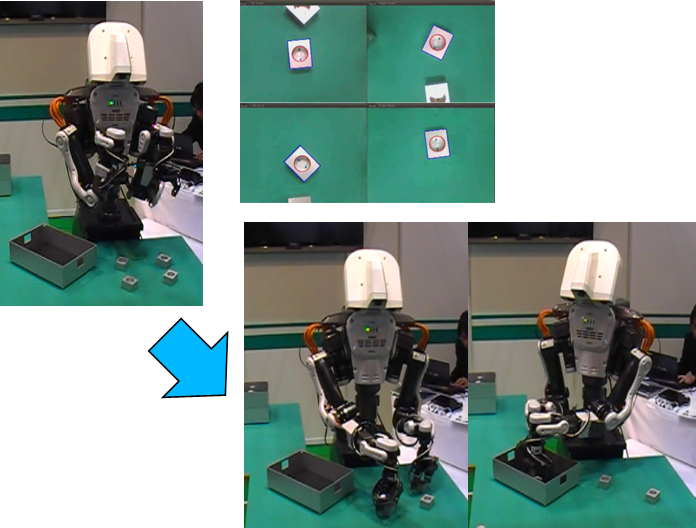
\includegraphics[width=0.8\linewidth]{figure/system.png}
  \caption{$B%5!<%S%9%$%a!<%8(B}
  \label{fig:system}
 \end{center}
\end{figure}
\begin{figure}[htb]
 \begin{center}
  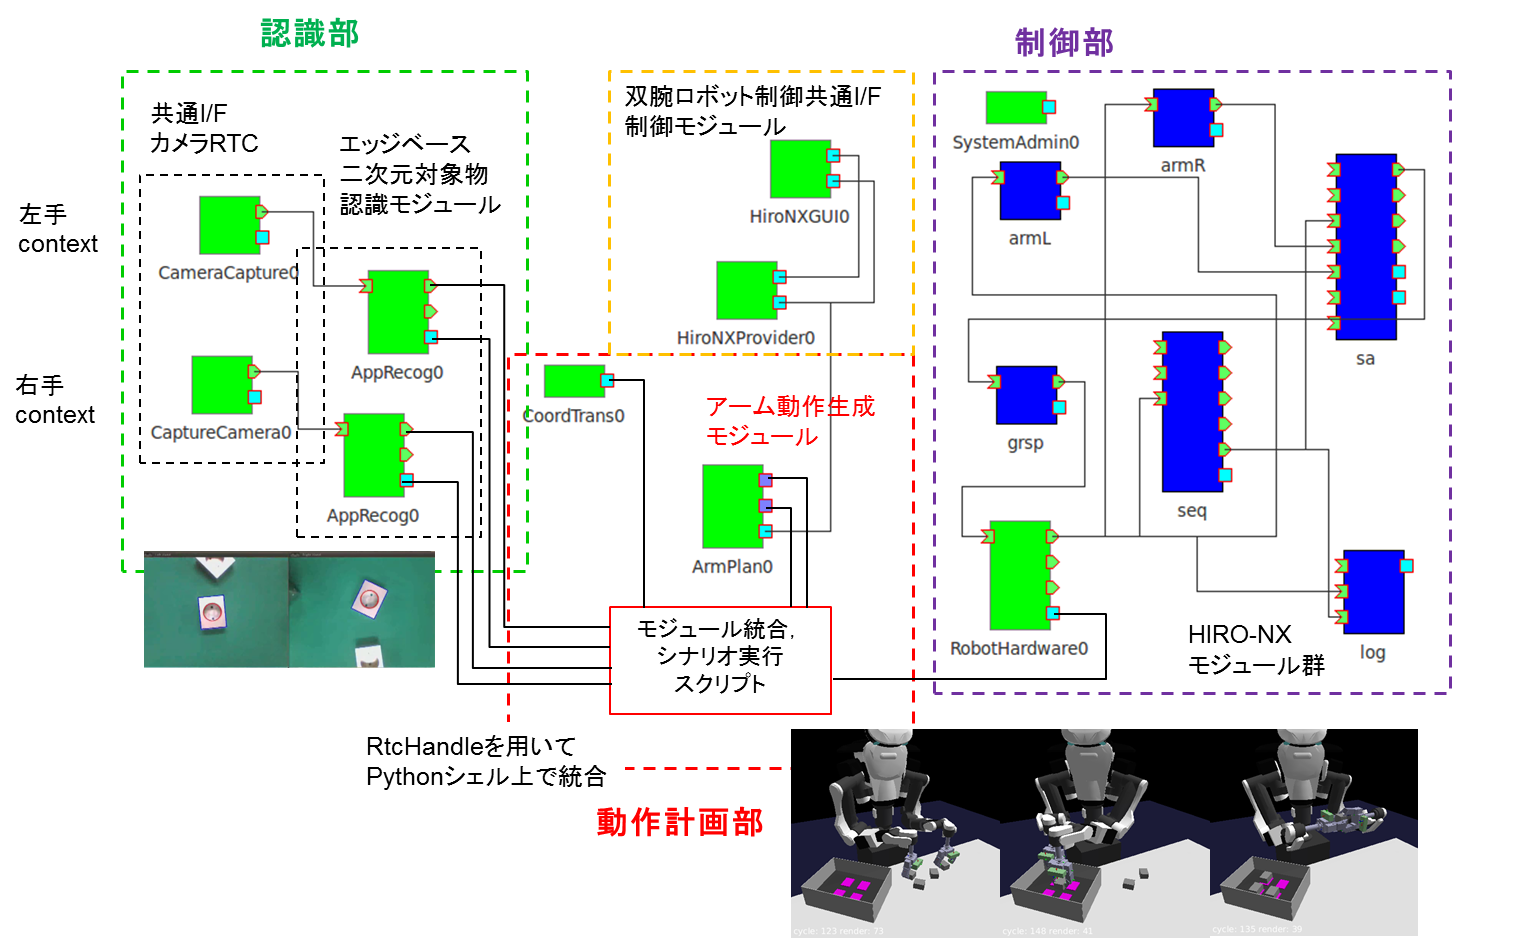
\includegraphics[width=1.0\linewidth]{figure/rtc_diagram.png}
  \caption{$BA4BN$N%b%8%e!<%k9=@.(B}
  \label{fig:rtc_diagram}
 \end{center}
\end{figure}


\section{$BG'<1It(B}

\subsection{$B%(%C%8%Y!<%9Fs<!85BP>]J*G'<1%b%8%e!<%k(B(AppRecog)}

http://openrtm.org/openrtm/ja/project/NEDO\_Intelligent\_PRJ\_HiroAccPrj\_5002

HiroNX$B$N<j@h$K<h$jIU$1$i$l$?(BUSB$B%+%a%i$GBP>]J*$rG'<1$9$k$?$a$N%b%8%e!<%k(B
$B$G$"$k!%%+%a%i%Q%i%a!<%?$O%G!<%?%]!<%H$rDL$7$F2hA|$H0l=o$KAw$i$l$F$/$k$b(B
$B$N$rMxMQ$9$k!%@5$7$$%+%a%i%Q%i%a!<%?$,F~$C$F$$$J$/$F$bBP>]J*$NG'<1$O$G$-(B
$B$k$,!$0LCV$*$h$S;Q@*$O@5$7$/?dDj$5$l$J$$!%(B

\subsubsection{$B%@%&%s%m!<%I$H%3%s%Q%$%k(B}

\begin{itemize}
 \item $B8=>u$G$O(Bgoogle code(SVN)$B$+$i3+H/HG$r%A%'%C%/%"%&%H(B
 \item $B$I$3$+$N%P!<%8%g%s$N(Btar$B$r:n$kM=Dj(B
\end{itemize}

\begin{lstlisting}
 $ cd app-recog
 $ make
\end{lstlisting}

\subsubsection{$B3+H/!&F0:n4D6-(B}

\begin{itemize}
 \item Ubuntu Linux 10.04 LTS
 \item OpenRTM-aist 1.0.0-RELEASE C++$BHG(B
 \item OpenCV 2.3
\end{itemize}

\subsubsection{$B%$%s%?%U%'!<%9(B}

\begin{itemize}
 \item $B%G!<%?%]!<%H(B
       \begin{itemize}
	\item $BF~NO(B: Img::TimedCameraImage (Img.idl) \\
	      $B2hA|=PNO6&DL%$%s%?%U%'!<%9=`5r$N%+%a%i%b%8%e!<%k$+$i!$(B
	      $B2hA|5Z$S!$%+%a%i%Q%i%a!<%?$r<u<h$j$^$9!%(B
	\item $B=PNO(B: TimedRecognitionResult (Vision.idl) \\
	      $BG'<17k2L6&DL%$%s%?%U%'!<%9$K$7$?$,$$!$BP>]J*BN$N0LCV;Q@*$r=PNO$7$^$9!%(B
	      Img::TimedCameraImage $B=hM}7k2L$r2hA|$H$7$F=PNO$7$^$9!%(B
       \end{itemize}
 \item $B%5!<%S%9%]!<%H(B \\
       $BG'<1BP>]$N%b%G%k$r@_Dj$9$k$?$a$K;H$$$^$9!%(B
       $B$"$i$+$8$a!%(BModelFiles/ModelList.txt$B$K%b%G%k(BID$B$H%b%G%kDj5A%U%!%$(B
       $B%kL>$r5-=R$7!$%b%G%k(BID$B$r0z?t$H$7$F%5!<%S%9%3!<%k$r9T$$$^$9!%(B
       setModelID(i)$B$O!$(Bi$BHV$N%b%G%k$r;HMQ$9$k$3$H$r0UL#$7$^$9!%(B
\end{itemize}
 $BG'<17k2L$O(BTimedRecognitionResult$B$K$h$C$F=PNO$5$l$^$9!%(B
 $B6qBNE*$J=PNOFbMF$O0J2<$NDL$j$G$9!%8=:_!$BP>]J*$N;Q@*0J30$OF~$C$F$$$^(B
 $B$;$s!%(B
\begin{verbatim}
  0: 0, 1: 0, 2: 0, 3: 0, 4: 0
  5: 0, 6: 0, 7: 0, 
  8: R00,  9: R01, 10: R02, 11: Tx
 12: R10, 13: R11, 14: R12, 15: Ty
 16: R20, 17: R21, 18: R22, 19: Tz
\end{verbatim}

\subsubsection{$B%+%9%?%^%$%:(B}

$BO"B3E*$KAw$i$l$F$/$k2hA|$KBP$7$FG'<1$r9T$$$^$9$,!$G'<17k2L$N;~4VJ}8~$NO"B3@-(B
$B$O9MN8$;$:!$3F%U%l!<%`$G0lHVL`EY$,9b$$0LCV$r7W;;$7!$$=$NL`EY$,ogCM0J>e$G(B
$B$"$l$P8!=P7k2L$rJV$7$^$9!%(B

% $BG'<1<jK!$N4JC1$J@bL@(B
% $BogCM$N0UL#$K$D$$$F(B
% $B%5!<%S%9$K$h$kG'<1BP>]$N@Z$jBX$((B
% $BG'<1%b%8%e!<%k$K$*$1$kBP>]J*%b%G%k$NDj5A$N;EJ}(B

$B%b%G%k$H<B2hA|$N%^%C%A%s%0$O!$$O2hA|:BI87O$G9T$o$l$^$9!%8!=P$7$?0LCV!$;Q(B
$B@*!$%9%1!<%k$+$i%+%a%i%Q%i%a!<%?$rMQ$$$F!$%+%a%i:BI87O$K$*$1$kBP>]J*$N0L(B
$BCV!$;Q@*$,7W;;$5$l$^$9!%(B
$B$7$?$,$C$F!$2hA|:BI8$G$N(B$(x,y,\theta)$$B$NC5:wHO0O!$8!=P$NogCM$r%3%s%U%#%0(B
$B%U%!%$%k(BAppRecog.conf$B$G;XDj$7$^$9!%(B
$B$^$?!$%b%G%kDj5A%U%!%$%k$O(B./ModelFile$B$NCf$KCV$-!$%U%!%$%k$OD:E@$HJU$K$h$C(B
$B$F9=@.$5$l$F$$$^$9!%(B

\begin{figure}[tb]
 \begin{center}
  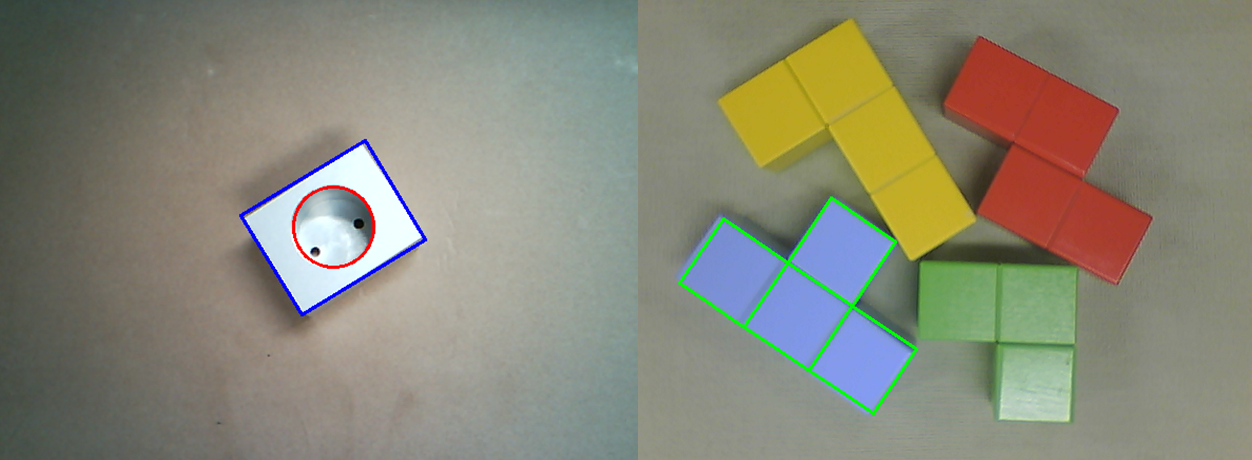
\includegraphics[width=0.8\linewidth]{figure/apprecog.png}
  \caption{$BG'<1Nc(B}
  \label{fig:apprecog}
 \end{center}
\end{figure}

\subsection{$B%+%a%i6&DL(BI/F$B=`5r$N2hA|%-%c%W%A%c%b%8%e!<%k(B(CameraComp)}

http://www-arailab.sys.es.osaka-u.ac.jp/CameraIF/

$BBg:eBg3X$K$h$j3+H/$5$l2hA|%-%c%W%A%c%b%8%e!<%k(BCameraComp$B$r%@%&%s%m!<%I!$(B
$B%3%s%Q%$%k$9$k!%%m%02hA|$K$h$k%F%9%H$r9T$&$?$a!$(BLoadPictureComp$B%b%8%e!<(B
$B%k$bF1MM$K%@%&%s%m!<%I$9$k$H$h$$!%(B


\subsection{$BG'<1It$NF0:n3NG'(B}

$B<B:]$K%+%a%i%b%8%e!<%k$H@\B3$7!$%*%s%i%$%s$G%F%9%H$r9T$&!%(B
$B$3$N$H$-$N%b%8%e!<%k@\B3$O(B\figref{fig:test_by_camera}$B$N$h$&$K$J$j!$(B
$B<B9T<j=g$O!$0J2<$NDL$j$G$"$k!%(B
\begin{enumerate}
 \item $BG'<1%b%8%e!<%k(BAppRecog$B$H%-%c%W%A%c%b%8%e!<%k$r$=$l$>$l<B9T$9$k!%(B
 \item rtshell$B$G2hA|$NF~=PNO$r@\B3$9$k(B(system editor$B>e$GA`:n$7$F$b$h$$(B)$B!%(B
 \item 2$B$D$N(BRTC$B$r(Bactivate$B$9$k!%(B
\end{enumerate}

\begin{lstlisting}
 $ cd CameraComp
 $ ./CaptureCameraComp
 $BJLC<Kv$G(B
 $ cd app-recog/
 $ build/bin/AppRecogComp
 $BJLC<Kv$G!J(Brtctree$B$G$N%Q%9$OE,Ev$KJd40$9$k!K(B
 $ rtcon CaptureCamera0.rtc:CameraImage AppRecog0.rtc:InputImage
 $ rtact CaptureCamera0.rtc AppRecog0.rtc
\end{lstlisting}

$B=i4|@_Dj$GG'<1HO0O$N%9%1!<%k$r9J$C$F$"$k$?$a!$G'<1$G$-$J$$>l9g$O(B
$BBP>]J*$^$G$N5wN%$r$$$m$$$mJQ$($F$_$k!%(B
$B$^$?!$GX7J$KLOMM$,$J$/!$BP>]J*$H0[$J$k?'$N$b$N$rCV$/$HG'<1$7$d$9$/$J$k!%(B

$B%F%9%H$H$7$F!$%+%a%i%b%8%e!<%k$r(BLoadPictureComp$B%b%8%e!<%k$K:9$7BX$(!$(B
$B$"$i$+$8$a;#$C$F$*$$$?2hA|$rMQ$$$F%F%9%H$r9T$&>l9g!$(B
CaptureCameraComp$B$r(BLoadPictureComp$B$KCV$-49$($?@\B3$H$J$k!%(B
$B%m%02hA|$N;XDj$O!$(BLoadPictureComp$B%b%8%e!<%k$N(BLoadPicture.conf$B$G(B
$B9T$&!%(BAppRecog$B%b%8%e!<%kIUB0$N2hA|(Bdata/parts4.jpg$B$rMQ$$$F3NG'$r9T$&$H$h(B
$B$$!%(B
$B>uBV6u4V$K$*$1$kC5:wHO0O$OJLES;XDj$,2DG=$G$"$k!%(B

% \begin{figure}[tb]
%  \begin{center}
%   %\includegraphics[width=0.5\linewidth]{figure/recog_test_log.png}
%   \caption{$B%m%02hA|$rMQ$$$?%F%9%H(B}
%   \label{fig:test_by_image}
%  \end{center}
% \end{figure}

\begin{figure}[tb]
 \begin{center}
  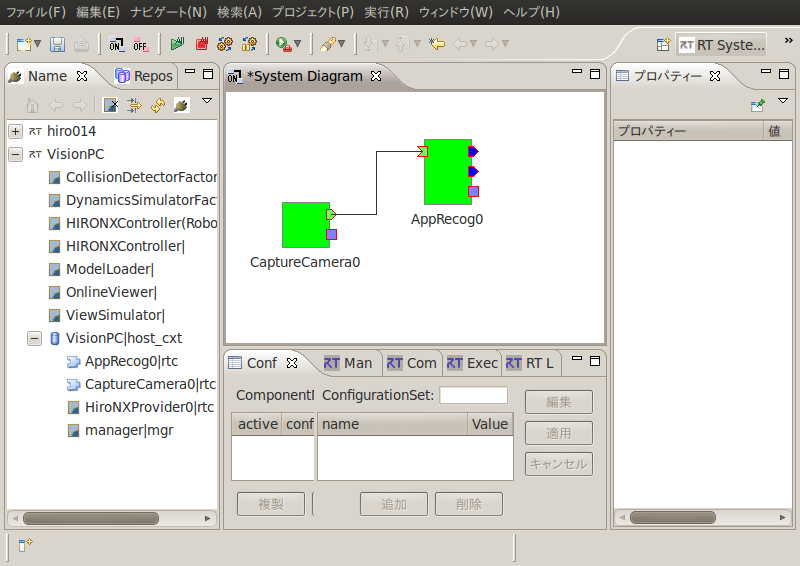
\includegraphics[width=0.8\linewidth]{figure/recog_test_cam.png}
  \caption{USB$B%+%a%i$rMQ$$$?%F%9%H(B}
  \label{fig:test_by_camera}
 \end{center}
\end{figure}


\section{$BF0:n@8@.It(B}

\subsection{(VPython$BHG(B)HiroNX$BF0:n@8@.%b%8%e!<%k(B}

http://openrtm.org/openrtm/ja/project/NEDO\_Intelligent\_PRJ\_HiroAccPrj\_5003

Python$BBPOC4D6-$K$*$$$F!"4v2?%b%G%k$rMQ$$$?F0:n@8@.%7%9%F%`$r=@Fp$K9=C[$9$k$?$a$N(B
$B%9%/%j%W%H72$G$9!%(BRtcHandle$B$rMQ$$$FBPOC4D6-$+$i(BRTC$B9=@.$K$h$k%7%9%F%`$N(B
$B3F%b%8%e!<%k$HDL?.$r9T$&$3$H$G!$%7%9%F%`$NE}9g$r9T$$$^$9!%(B
RRT-connect$B$K$h$kAPOS$N43>D$r9MN8$7$?F0:n7W2h5!G=$rDs6!$7!$?M<j$K(B
$B$h$kF0:n5-=R$H%W%i%s%J$K$h$kF0:n@8@.$r%9%`!<%:$KE}9g$G$-$^$9!%(B
$B$^$?!$(BRTC$B$H$7$F!$:n6H6&DL%$%s%?%U%'!<%9$r<BAu$9$kF0:n@8@.%b%8%e!<%k$H$7(B
$B$FMxMQ$9$k$3$H$b$G$-$^$9!%(B

\subsubsection{$B%@%&%s%m!<%I$H%3%s%Q%$%k(B}


\begin{lstlisting};
 $ cd iv-plan-hironx/iv_plan/scripts; ./install-debs.sh
 $ cd iv-plan-hironx/iv_plan/; make
 $B4D6-JQ?t(BPYTHONPATH$B$K(B iv-plan-hironx/iv_plan/src$B$rDI2C(B
\end{lstlisting}

$B4D6-$K$h$C$F(BVPython$B$,@5$7$/F0:n$7$J$$>l9g$,$"$k$?$a!$$^$?!$(Bdeb$B%Q%C%1!<%8(B
$B$G%$%s%9%H!<%k$5$l$k%P!<%8%g%s$G$O%5%]!<%H$5$l$F$$$J$$5!G=$rMxMQ$9$k$?$a!$(B
VPython$B$O(BUbuntu 10.04LTC$B$NI8=`%Q%C%1!<%8$h$j?7$7$$$b$N$K%Q%C%A$rEv$F!$%3(B
$B%s%Q%$%k:Q$_$N$b$N$rMxMQ$7$^$9!%$3$l$O!$(Bmake$B;~$K%@%&%s%m!<%I$7$^$9!%(B
$B$7$?$,$C$F!$I8=`$N(Bpython-visual$B%Q%C%1!<%8(B
$B$r%$%s%9%H!<%k$7$F$$$k>l9g$O!$$=$l$,(Bpython$B>e$G@h$K%m!<%I$5$l$k$3$H$,$J$$(B
$B$h$&$KCm0U$9$kI,MW$,$"$j$^$9!%(B
ikfast$B$K$h$j@8@.$5$l$?(BHIRO-NX$BMQ5U1?F03X7W;;$N%=!<%9$OF1:-$5$l$F$*$j!$(BPQP
$B$N%=!<%9$O(Bmake$B;~$K%@%&%s%m!<%I$7!$$=$l$>$l%3%s%Q%$%k$5$l$^$9!%(B
$B$=$l0J30$KI,MW$J$b$N$O(Bapt$B%3%^%s%I$G%$%s%9%H!<%k$7$^$9(B(install-deb.sh).

\subsubsection{$B3+H/!&F0:n4D6-(B}

\begin{itemize}
 \item Ubuntu Linux 10.04 LTS 32bit/64bit
 \item OpenRTM-aist 1.0.0 (Python$BHG(B)
\end{itemize}

\subsubsection{$B4pK\E*$J;H$$J}(B}

$B$^$:!$%?%9%/5-=R!$F0:n7W2h!$G'<1$*$h$S@)8f%b%8%e!<%k$H$N@\B3$r(B
$B#1$D$N(BPython$B%7%'%k>e$G9T$&J}K!$r@bL@$7$^$9!%(B

\begin{lstlisting}[label=src:branch]
 $ cd iv_scenario/src
 $ ipython test.py
 >>> test1()

 $BN)BN%Q%:%k%G%b(B
 $ ipython puzzle.py
 >>> demo() # $B%Q%:%kG[CV$r85$KLa$9$N$O(B reset_puzzle()

 $B%7%_%e%l!<%7%g%s$K$h$kItIJ$NH"5M$a(B
 >>> $BJQ99Cf(B
\end{lstlisting}

$B%&%#%s%I%&A`:n$O!$1&%I%i%C%0$G2sE>!$Cf%I%i%C%0$G%:!<%`$G$9!%(B
$B%W%m%0%i%`$N=*N;$O(BCtrl+d$B$G%$%s%?!<%W%j%?$rH4$1$?8e!$(BGUI$B$NJD$8$k%\%?%s$r(B
$B2!$7$^$9!%(BCtrl+c$B$O%H%i%C%W$5$l$F$$$^$9!%(BGUI$B$NJD$8$k%\%?%s$r2!$9$N$,LLE](B
$B$J>l9g$O(BCtrl+\textbackslash $B$G(BSIGQUIT$B$rAw$k$3$H$G=*N;$5$;$k$3$H$,$G$-$^$9!%(B

Python$B%7%'%k>e$G%m%\%C%H$N;Q@*$rJQ99$7$?$j!$4D6-Cf$NJ*BN$r0\F0$5$;$?$j!$(B
$BF0:n7W2h$r9T$&>l9g$NA`:n$K4X$7$F$OIUO?$r;2>H$7$F$/$@$5$$!%(B

$B30It(BRTC$B$H$NDL?.$K$O(BRtcHandle$B$rMxMQ$7$F$$$^$9!%(B
(http://staff.aist.go.jp/t.suehiro/rtm/rtc\_handle.html)

$B4pK\E*$K!$%m%\%C%H%/%i%9!$%m%\%C%H%$%s%9%?%s%9$4$H$N%+%9%?%^%$%:$O(B
$B4{B8%/%i%9$r3HD%$9$k$3$H$G9T$$$^$9!%(B
\begin{itemize}
 \item robot.py$B$+$i(Bhironx.py
 \item hironx\_params.py
       $B8DBN:9$,$"$k3F<o(Btransform$B$H!$MxMQ$9$k30It%b%8%e!<%kDj5A(B
 \item $B4D6-%b%G%k$NDj5A(B \\
       (python$B$N%G!<%?9=B$$GM?$($k!%(Bscene\_object.py)
 \item $BB>$N5!G=$H$7$F!$(BVRML$B$N%m!<%@!$%;%s%5<h$jIU$10LCV$N?dDj5!G=$,$"$j(B
       $B$^$9(B.
\end{itemize}


\begin{figure}[tb]
 \begin{center}
  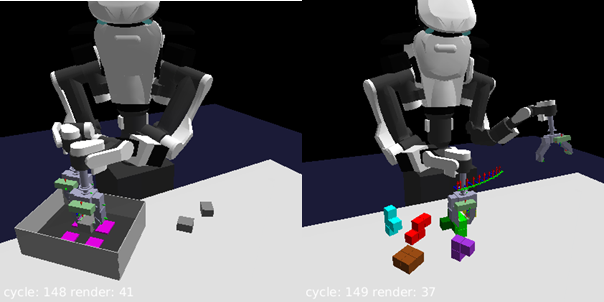
\includegraphics[width=0.8\linewidth]{figure/planner_scripts.png}
  \caption{$BF0:n@8@.%b%8%e!<%k(B}
  \label{fig:planner_scripts}
 \end{center}
\end{figure}

\subsubsection{$B%$%s%?%U%'!<%9(B}


\subsection{HiroNXInterface}

http://www.openrtm.org/openrtm/en/node/4645

$BAPOS%m%\%C%H$N@)8f%3%^%s%I$N6&DL%$%s%?%U%'!<%9$K=`5r$9$k(B
HiroNX$BMQ@)8f%b%8%e!<%k$G$9!%(B
$B>\:Y$K$D$$$F$O!$3+H/85$G$"$k;:6H5;=QAm9g8&5f=j$N%I%-%e%a%s%H$r;2>H$7$F$/(B
$B$@$5$$!%(B

\subsection{$BF0:n@8@.It$NF0:n3NG'(B}

 % $ $B5/F0%9%/%j%W%H(B
 % IP/$B%[%9%HL>$N0c$$$O$I$3$rD>$;$P$h$$$+!)(B

$B0J2<$N%3%^%s%I$G%G%b%W%m%0%i%`$r5/F0$7$^$9!%(B

\begin{lstlisting}[label=src:branch]
 $ cd iv_scenario/src
 $ ipython demo_wexpo.py

 $B%7%_%e%l!<%7%g%s$G$N%G%bF0:n$N<B9T(B
 >>> demo(False)

 $B30It%b%8%e!<%k$H$NDL?.(B
 (AppRecog$B%b%8%e!<%k$r<B9T$7$F$*$/(B)
 >>> rr.detect(sensor='rhandcam') # $B1&<j%O%s%I%+%a%i$G$NG'<1(B

 $B0J2<$O!$(BHiroNX$B$N5/F0$,40N;$7!$(BHiroNX$BBNFb$N%b%8%e!<%k$HDL?.2DG=$J>uBV$G(B
 $B$"$k$H$9$k!%(B
 >>> detect(sensor='rhandcam') # $BG'<17k2L$r@$3&:BI8$KD>$7$?$b$N(B
 >>> rr.get_joint_angles() # $B<B5!$N4X@a3QEYNs(B
 >>> r.prepare() # $B%7%_%e%l!<%?Fb$G;Q@*$rJQ99(B
 >>> sync() # $B<B5!$N;Q@*$r%7%_%e%l!<%?$K$"$o$;$k(B
\end{lstlisting}


\subsection{$BF0:n@8@.$rBPOC4D6-$G9T$&>l9g(B}

\subsection{$BF0:n@8@.$rF0:n7W2h%b%8%e!<%k$H$7$FJ,N%$9$k>l9g(B}

$B%7%_%e%l!<%7%g%s4D6-(B
$B30It%b%8%e!<%k$H$NDL?.(B
$BF0:n%3%^%s%IAw?.!$>uBVFI$_9~$_(B

\chapter{$B=`Hw(B}

$BI,MW$K1~$8$F9T$&%m%\%C%H$4$H$K0J2<$N:n6H$r9T$&!%(B

\section{$B%b%G%k%U%!%$%k$N=$@5!JNO%;%s%5$"$j$H$J$7!K(B}


\section{$B%-%c%j%V%l!<%7%g%s(B}

$B%m%\%C%H$N8DBN:9$r=$@5$9$k:n6H$G$"$k!%(B
$B%G%U%)%k%HCM$O(BHiroNX16$B9f5!$N$b$N$G$"$j!$(B
$B@:EY$r=P$9$K$O3F5!BN$4$H$K9T$&I,MW$,$"$k!%(B

\subsection{$B%+%a%i%-%c%j%V%l!<%7%g%s(B}

RT-middleware$B$N%3%s%]!<%M%s%H$G$b(BROS$B$N%N!<%I$G$b2?$G$b$h$$$N$G(B
$BC14c%+%a%i$N%-%c%j%V%l!<%7%g%s$r9T$$!$(BCameraComp$B$,FI$_9~$a$k$h$&$K(B
$B$9$k!%(B

$B$=$N8e!$%(%C%8%Y!<%9Fs<!85BP>]J*G'<1%b%8%e!<%k$K$*$$$F!$BP>]J*$N0LCV!$5w(B
$BN%$,@5$7$/=PNO$5$l$F$$$k$+$I$&$+3NG'$7$F$*$/$H$h$$!%(B

\subsection{$B%+%a%i<h$jIU$10LCV$N%-%c%j%V%l!<%7%g%s(B}

$B8=>u$G$O!$%A%'%C%+!<%\!<%I$NG'<1$K(BROS$B$N%N!<%I$r;HMQ$7$F$$$k!%(B
$B%-%c%j%V%l!<%7%g%s%W%m%0%i%`$O!$3X=,%G!<%?$H$7$F%m%\%C%H$N3F;Q@*$K$*$1$k(B
$B%A%'%C%+!<%\!<%I$N;Q@*$rF~NO$H$7$^$9!%%A%'%C%+!<%\!<%I$N;Q@*$O(Btf$B$H$7$F(B
publish$B$5$l$?%a%C%;!<%8$r(Bpython$B%W%m%0%i%`$G<u?.$7$^$9!%(B
$B$7$,$C$F!$=`Hw$H$7$F!$(B
\begin{itemize}
 \item ROS$B$N%+%a%i%N!<%I$K$h$j2hA|$*$h$S>e5-%+%a%i%Q%i%a!<%?$,%H%T%C%/$H(B
       $B$7$F(Bpublish
 \item checkerboard detection$B%N!<%I$G$=$l$i$r(Bsubscribe$B$7!$?dDj$7$?(Btf$B$,(Bpublish
\end{itemize}
$B$5$l$k>uBV$K$7$F$*$/I,MW$,$"$j$^$9!%(B

\subsubsection{$B<j=g(B}

\begin{lstlisting}
 1, $B4y$N>e$K%A%'%C%+!<%\!<%I$rCV$/(B

 2, $B<s$rF0$+$7$F3X=,%G!<%?$r$H$k(B
 $ ipython hironx_calib.py
 >>> res = record_data()  
 # $B<j@h$rF0$+$7$F2hA|$H$=$N$H$-$N4X@a3QEYCM$r<hF@$9$k(B.
 # $B$9$Y$F$N;Q@*$G%A%'%C%+!<%\!<%I$,;kLn$KF~$j!$(B
 # $B0BDj$7$FG'<1$G$-$F$$$k$+$I$&$+$r3NG'$9$k!%(B

 3, $BF,%j%s%/$+$i(Bkinect$B%+%a%i$X$N(Btransform$B$r7W;;$9$k(B
 >>> f = calibrate(res, height=960.0)

 4, transform$B$N=q$-49$((B
 >>> r.Thd_kinectrgb = f

 5, $B3NG'!J@5$7$$0LCV$G%-%c%j%V%\!<%I$N%U%l!<%`$,;_$^$C$F$$$l$P@.8y!K(B
 >>> play_data(res)

 6, $B%G%U%)%k%HCM$N99?7(B
 hironx_params.py$B$N(BThd_kinectdepth$B$r=q$-49$($k(B
\end{lstlisting}

\begin{itemize}
 \item $B>e$N%3%^%s%I$OF,It(Bkinect$B$N>l9g$J$N$G!$%O%s%I%+%a%i$N>l9g$KJQ99$9(B
       $B$k(B
 \item $B86M}$K$D$$$F(B
\end{itemize}

\chapter{$B%G%b$N<B9T(B}

\section{$BG'<1It$N%b%8%e!<%k5/F0$H@\B3(B}

VisionPC$B$K$F!$(Brun.sh$B$r<B9T$9$k!%(B
$B$3$l$K$h$j!$N><j$KBP1~$9$k%+%a%i!$G'<1%b%8%e!<%k!$(BHiroNXInterface$B@)8f%b(B
$B%8%e!<%k$,5/F0!$@\B3$5$l!$$5$i$K3F%b%8%e!<%k$,(Bactivate$B$5$l$^$9!%(B
HiroNXInterface$B%b%8%e!<%k$O5/F08e(BGUI$B>e$N!V(BRTC Status$B!W$,NP$K$J$C$?>uBV$G(B
$B!V(BSet up Robot$B!W%\%?%s$r2!$7(BRTC$B$^$o$j$N=i4|2=$r9T$&I,MW$,$"$kE@$KCm0U$7(B
$B$F$/$@$5$$!%(B

$B$3$3$G!$(Brtc.conf,$B:81&%+%a%i$N:81&$N%+%a%i$,5U$K$J$C$F$$$J$$$+$I$&$+3NG'(B
$B$7$F$/$@$5$$!%(B

\section{$BF0:n@8@.%W%m%0%i%`$N5/F0(B(1$B$D$N(Bpython$B%W%m%;%9>e$G$N<B9T(B)}

\begin{itemize}
 \item $B%F!<%V%k>e$KBP>]J*$r(B4$B$DG[CV$7!$(B
       look\_for()$B4X?t$r<B9T$7$^$9!%(B
       $B<j@h$rF0$+$7$F4y>e$NBP>]J*$rG'<1$7$F$_$^$9!%(B
 \item $B$3$N$H$-!$2hA|Cf$GBP>]J*$,@5$7$/G'<1$5$l$F$$$k$+!$G'<17k2L$,%7%_%e(B
       $B%l!<%?Cf$K@5$7$/I=<($5$l$F$$$k$+$I$&$+$r3NG'$7$^$9!%(B
 \item $B$3$l$G=`Hw$,@0$C$?$N$G!$<B:]$K%G%b$r<B9T$7$^$9!%(B
       $B<B9T8e!$%m%\%C%H$O%F!<%V%k$r%9%-%c%s$7!$BP>]J*$rG'<1(B
       demo()
\end{itemize}


\appendix
\chapter{VPython$B4D6-$G$N%W%m%0%i%_%s%0(B}

$B%U%l!<%`$d%m%\%C%H!$4D6-Cf$NJ*BNA`:nEy$r(Bpython$B>e$G9T$&J}K!$K$D$$$F@bL@$7(B
$B$^$9!%(B

$B0J2<$N>pJs$O8E$$$b$N$G!$99?7M=Dj$G$9!%(B

\begin{verbatim}

# 0, $B$O$8$a$K(B

$ roscd MotionPlan/src
$ ipython demo.py


# 1, python$B$r;H$&(B

dir(r) # $B4X?t$d%a%=%C%I$N0lMw(B
r. [TAB] # $B%a%=%C%IL>Ey$NJd4V!J(Bipython$B$N5!G=!K(B
help(r) # $B0z?t$d@bL@(B

# $B$H$j$"$($:%G%b(B

putbox() # $BH"$rG'<1$7$FDO$_!"CV$-D>$9(B
putbox(name='box1')
demo()

demo2() # $B:8<j$G$N%"%W%m!<%A(B

qs = gen_traj() # $B<j@h$G(Bsin$B%+!<%V$rIA$/$?$a$N4X@a3Q50F;$r:n$k(B
play_traj(qs) # $B:n$C$?50F;$r<B9T$9$k(B

# $B%3%^%s%I%i%$%s(B
# Ctrl+c
# Ctrl+p / Ctrl+n
# Ctrl+r


# 2, $B4D6-Cf$NJ*BNA`:n(B

env
env.get_objects() # $B4D6-Cf$NJ*BN0lMw(B
[x.name for x in env.get_objects()] # $BJ*BNL>0lMw(B

# $BJ*BN$OL>A0$G4IM}$5$l$F$$$k!#(B
# $BF1$8L>A0$NJ*BN$ODI2C$G$-$J$$$N$G!"0lEY:o=|$9$k$+!"L>A0$rJQ$($FDI2C$9$k!#(B
putbox() # $B%F!<%V%k>e$KH"$rCV$/(B
b = env.get_object('box') # $BL>A0$GJ*BN<hF@(B
put_box(name='box2') # $BL>A0$rJQ$($k$H0c$&J*BN(B
env.delete_object('box2')

frm = b.where() # $BJ*BN$N0LCV$H;Q@*$r<hF@(B

# $B%m%\%C%H$N0\F0!"2sE>(B ( world=>basejoint$B$N:BI8JQ49$NJQ99(B )
r.go_pos(-150,500,0) # 2D$B:BI8(B, (x,y,theta)
r.go_pos(-150,0,pi/2) # $B2#$r8~$/(B


# 3, $B<+:n%5%s%W%k$N=q$-J}(B
emacs mysample.py

== mysample.py ==
from demo import *

... $BE,Ev$J%3!<%I(B ...
== ==

ipython mysample.py

# $B%5%s%W%k$r=$@58e$O!"0J2<$r<B9T$9$k$H(B
# mysample.py$B$N=$@5$,H?1G$5$l$k(B

import mysample # $B:G=i$N0l2s$@$1(B

reload(mysample)
from mysample import *


# 4, $B%m%\%C%H$N;Q@*$NA`:n(B

# joint, link$B$N<hF@(B
r
r.get_joints()
r.get_links()

# $B%8%g%$%s%HL>$N<hF@(B
j0 = r.get_joints()[0]
dir(j0)
j0.angle
j0.name
map(lambda x: x.name, r.get_joints())
[x.name for x in r.get_joints()]

# $B4X@a3QEY$NI=<((B
r.get_joint_angles()
# $B$3$l$O2<$N%3!<%I$HF1$8(B
[x.angle for x in r.get_joi

# $BOS$@$1(B
r.get_arm_joint_angles()
r.get_arm_joint_angles(arm='left')
r.set_arm_joint_angles(angles)
r.set_arm_joint_angles(angles, arm='left')

# $B%O%s%I$@$1(B
r.get_hand_joint_angles()
r.get_hand_joint_angles(hand='left')
r.set_hand_joint_angles(angles)
r.set_hand_joint_angles(angles, hand='left')

# $B4X@a#1$D$rJQ$($k(B
r.get_joint_angle(0) # ID
r.set_joint_angle(0, 0.5) # ID$B$H3QEY(B[rad]

# $B=i4|;Q@*$KLa$9(B
r.reset_pose()

# $B$"$i$+$8$a$$$/$D$+$N;Q@*$,Dj5A$5$l$F$$$k(B
r.poses
r.poses.keys()

# r.reset_pose()$B$O0J2<$HF1$8(B
r.set_joint_angles(r.poses['init'])

# $B<j$N%]!<%:(B
r.hand_poses
r.hand_poses['open']
r.set_hand_joint_angles(r.hand_poses['open']) # $B<j$r3+$/(B
r.set_hand_joint_angles(r.hand_poses['close']) # $B<j$rJD$8$k(B

# $B%"%K%a!<%7%g%s!J<s$r?6$C$F$_$k!K(B
arange(0, 1, 0.2)
for th in arange(0,1,0.2):
        r.set_joint_angle(1, th)
        time.sleep(0.5)

# $B$A$J$_$K:81&$NOS$N4X@a=q$/<hF@$O0J2<$N%3!<%I$HF1$8(B
r.get_joint_angles()[3:9]
r.get_joint_angles()[15:19]



# 5, $B:BI87O(B(frame)$B$K$D$$$F(B
# 3x3$B2sE>9TNs$H(B3$B<!85%Y%/%H%k(B = 4x4$B$NF1<!?t9TNs(B
# euler$B3Q(B, $B<+M3<42sE>(B, quaternion

help(VECTOR)
help(MATRIX)
help(FRAME)

# $BCM$N@8@.(B(constructor)
VECTOR()
MATRIX()
FRAME()
v=VECTOR(vec=[100,0,0])
MATRIX(angle=pi/2, axis=VECTOR(vec=[0,0,1]))
MATRIX(c=pi/2) # a,b,c$B$rF1;~$K;XDj$G$-$J$$$N$GCm0U(B
m=MATRIX([[1,0,0],[0,1,0],[0,0,1]])
FRAME()

frm.mat # $B;Q@*ItJ,(B
frm.vec # $B0LCVItJ,(B

# $B1i;;(B
v*v # $B%Y%/%H%k@Q(B
dot(v,v) # $BFb@Q(B
v+v # $BOB(B
2*v # $B%9%+%i!<G\(B
# $B9TNs$O;Q@*I=8=@lMQ!JD>9T9TNs!K(B
m*m # $B@Q(B
-m # $B5U9TNs(B
# -m$B$O$8<BAu$OE>CV9TNs(B
# $B%9%+%i!<G\!"9TNsOB$ODj5A$5$l$J$$(B($BG[Ns$N7k9g2r<a$5$l$k(B)

# $B;Q@*I=8=4V$NJQ49(B
m.abc() # $B9TNs(B=>euler
m.rot_axis() # $B9TNs(B=>$B<+M3<42sE>(B
# euler=>$B2sE>9TNs!"<+M3<42sE>(B=>$B2sE>9TNs$O>e5-$N(BMATRIX$B$N%3%s%9%H%i%/%?(B

# $B0LCV$H;Q@*$r9g$o$;$?I=8=!JF1;~9TNs!K(B
FRAME(mat=m, vec=v)
FRAME(xyzabc=[x,y,z,a,b,c])

f=FRAME(vec=[500,0,1000])
show_frame(f)
f.mat = MATRIX(a=pi/4)
show_frame(f)

f.mat = MATRIX(a=pi/4)*MATRIX(b=pi/4)
show_frame(f)

# $B:BI87O$N?F;R9=B$(B
FRAME.affix() # $B:BI87O$N?F;R4X78$NDj5A(B
FRAME.unfix() # $B:BI87O$N?F;R4X78$N:o=|(B
FRAME.set_trans() # $B?F;R4V$N:BI8JQ49$N@_Dj(B
f.rel_trans # $B?F;R4V$N:BI8JQ49$N<hF@(B

# $BJ*BNDI2C(B
# putbox()$B$N5-=R$r;2>H(B
# $BI=<(MQ7A>u$H(BFRAME$B$r:n$j!"E,Ev$J?F:BI87O$N;R(BFRAME$B$H$7$F!":BI87O%D%j!<$KA^F~$9$k(B

env.insert_object('box2') # $BJ*BNDI2C(B
env.delete_object('box2') # $BJ*BN:o=|(B($B;R%U%l!<%`$NJ*BN$b:o=|$5$l$k(B)


# 6, $B5U1?F03X(B(Inverse Kinematics, IK)$B$NMxMQ(B

# $B<j<s0LCV!$;Q@*$N<hF@(B
r.fk() # $B=g1?F03X7W;;!$8=:_$N<j@h(BFRAME$B$rJV$9!%%G%U%)%k%H$O1&<j!%(B
r.fk(arm='left') # $B:8<j$OL@<(E*$K0z?t$G;XDj$9$k(B

# $BL\E*0LCV$X$N%"%W%m!<%A(B

putbox() # $B<j$,FO$-$=$&$J$H$3$m$KCV$/(B
objfrm = detect()

# $B%"%W%m!<%A;Q@*!$GD;};Q@*$N7W;;!J(B2$B$D$:$D5a$^$k!K(B
afrms, gfrms = pl.grasp_plan(objfrm)

# $B%"%W%m!<%A;Q@*$rI=<((B
# (FRAME$B$+$i(BCoordinateObject$B$r:n$C$F!"4D6-$K(Binsert_object$B$9$k(B)
show_frame(afrms[0])
show_frame(afrms[1])

# $BL\I80LCV$X<j$r?-$P$9$?$a$N4X@a3QEY$r7W;;$9$k(B
r.ik(afrms)
help(r.ik)
# - IK$B$OL\I8<j@h(BFRAME$B$N=89g$r0z?t$K$H$j!"(B
#   $B=i4|;Q@*$+$i4X@a6u4V$G$N=E$_IU$-5wN%=g$KJB$Y$?2r$NNs$rJV$9(B
#   $BL\I8<j@h%U%l!<%`#1$D$r0z?t$K;XDj$7$F$b$h$$(B
# - $B2r$,B8:_$7$J$1$l$P(BNone
# - $B$[$H$s$I$N>l9g!":G=i$N2r$r:NMQ$9$l$P$h$$(B

asols = r.ik(afrms)
r.set_arm_joint_angles(asols[0]) # $BOS$N3QEY$N$_(B

gsols = r.ik(gfrms)
r.set_arm_joint_angles(gsols[0]) # $BOS$N3QEY$N$_(B

# $B9x$r;H$&(B
# $B9x(Byaw$B<4$r;H$&$H<j$NFO$/HO0O$,Bg$-$/9-$,$k(B

asols = r.ik(afrms, use_waist=True) # $BJVCM$N7A<0$,0c$&$N$GCm0U(B (waist_yaw, arm_angles)
th,js = asols[0]
r.set_joint_angle(0,th) # $B9x$r2s$9(B
r.set_arm_joint_angles(js) # $BOS$N;Q@*$rJQ$($k(B

# $BB>$N2r$bI=<($7$F$_$k(B
for th,js in asols:
        r.set_joint_angle(0,th)
        r.set_arm_joint_angles(js)
        time.sleep(0.5)

# $BJ*BN$r%O%s%I$K8GDj$9$k(B
tgtobj = env.get_object('box0')
handjnt = r.get_joint('RARM_JOINT5')
reltf = (-handjnt.where())*tgtobj.where()
tgtobj.unfix()
tgtobj.affix(handjnt, reltf)

# $B<j@h50F;$G$NF0:n@8@.(B ($B<}B+(BIK$B$G$O$J$/!"=i4|;Q@*$K6a$$2r$rL@<(E*$KA*Br$7$F$$$k(B)

# $B50F;$N:n@.(B
traj = CoordinateObjects('trajectory')
traj.append( ... ) # $BE,Ev$J%U%l!<%`$rDI2C$9$k(B
env.insert_object(traj, FRAME(), env.get_world()) # $B@$3&:BI8AjBP$G50F;$rDj5A(B
traj.coords

# $B:o=|$7$?$$$H$-$O(B
env.delete_object('trajectory')

# 7, $B<B5!$rF0$+$9(B

# $B<B5!$H$N%$%s%?%U%'!<%9(B

rr = RealHIRO()
rr.connect() # $BG'<1=hM}$,;O$^$C$F$$$J$1$l$P3+;O;XNa$rAw$k(B
rr.get_joint_angles() # tf and joint state by ROS
js = r.get_joint_angles()
# socket(+pickle) to jython script
# scequencer, wait
duration = 4.0
rr.send_goal(js, 4.0) # blocking
rr.send_goal(js, 4.0, wait=False) # non-blocking
# blocking$B$J8F=P$7$b:GBg(B10[sec]$B$G(Btimeout$B$9$k;EMM(B

# $B<B:]$K$O!"%b%G%k$G;Q@*$r3NG'$7$F$+$i0J2<$r<B9T$9$k$N$,JXMx(B
sync() # $B%G%U%)%k%H$O(B4[sec]$B$G<B5!$r%b%G%k$KF14|$5$;$k(B
sync(duration=3.0) # $B;~4V$rJQ$($k(B

# $B%A%'%C%+!<%\!<%I$NG'<1(B
detect() # $BG'<17k2L$,(Bbox$B$H$7$FI=<($5$l$k(B
objfrm = detect() # $B<B5!$N>l9g$O(BROS$B$N<1JL4o$+$i(Btf$B$r<u?.(B
                  # simulation$B$N>l9g$OD>@\!"J*BN0LCV$rFI$`(B

# Link$B$K1h$C$?:BI8JQ49(B
# $BG'<17k2L$O!"%+%a%i(B=>$BBP>]J*$N:BI8JQ49$G$"$k$N$G!"(B
# $B@$3&:BI8(B=>$BBP>]J*$N:BI8JQ49$KD>$9(B
# detect()$B4X?t$NCf$G9T$C$F$$$k=hM}(B
r.Thd_leye # $BF,%j%s%/(B => $B:8L\%+%a%i$X$NJQ49(B
Tleye_obj = rr.detect()
Twld_hd = r.get_link('HEAD_JOINT1_Link').where()
Twld_obj = Twld_hd * r.Thd_leye * Tleye_obj


# $B<B5!$N>l9g(B
hand_cam_demo()

# $B%7%_%e%l!<%?$G<B9T$9$k$H$-$O!$@h$K<j$,FO$/>l=j$KH"$rCV$$$F$*$/(B
# 'box0' => marker 0, 'box1' => marker 1 $B$KBP1~(B
putbox(name='box0', vaxis='y')
putbox(name='box1', vaxis='y')
hand_cam_demo()

# $B$b$&0lEY<B9T$7$?$$$H$-(B
env.delete_object('box0')
putbox(name='box0', vaxis='y')


# $B%O%s%I%+%a%i$O(BAR-toolkit$B$K$h$k(Bmarker$BG'<1(B($BJ#?tJ*BNBP1~(B)
# $BJV$jCM$O(B ($B%^!<%+HV9f!"%+%a%i(B=>$B%^!<%+$N:BI8JQ49(B)$B$N%j%9%H(B
# non-blocking$B$G:G?7$NG'<17k2L$rJV$9(B
# $B2a5n(B thre [sec]$B0JFb$KG'<1$K@.8y$7$F$$$J$$%^!<%+$OJV$5$J$$(B
# $B%G%U%)%k%H$O(B thre = 0.5[sec]

lupus@ roslaunch Sense sense_lhand_ar.launch
rr.detect(camera='lhand') # $B:8<j%+%a%i$K$h$kG'<1(B

# $BJ?9T%0%j%C%Q$N4V3V;XDjGD;}(B
r.grasp(width=65, hand='right') # $B;X$N4V3V$,(Bwidth[mm]$B$K$J$k$h$&$K;X$rF0$+$9(B
r.grasp(65) # $B$3$l$G$bF1$8(B

# $B%"%W%m!<%A5wN%$N;XDj(B
pl.reaching_plan(objfrm, approach_distance=80) # $B>/$71s$/$+$i%"%W%m!<%A(B


# $BF0:n7W2h(B($B;EMM$,JQ$o$k2DG=@-Bg(B)
traj = test_plan() # RRT-connect$B$K$h$kF0:n7W2h(B
show_traj(traj) # $B50F;$NI=<((B
opttraj = pl.optimize_trajectory(traj) # $B50F;$N:GE,2=(B
show_traj(opttraj)
opttraj = pl.optimize_trajectory(opttraj) # $B$5$i$K%9%`!<%8%s%0(B

# $B43>D%A%'%C%/$K$O(BPQP$B$rMxMQ(B
# $B%m%\%C%H$N%b%G%k(BVRML$B$=$N$^$^(B

# $B43>D%A%'%C%/BP>]J*$NDI2CNc(B
r.add_collision_object(env.get_object('table top'))

\end{verbatim}

% \addcontentsline{toc}{chapter}{$B;29MJ88%(B}
% \markboth{$B;29MJ88%(B}{$B;29MJ88%(B}
% \bibliographystyle{junsrt}
% \bibliography{p2009}


\end{document}
